\documentclass{article}
\usepackage[utf8]{inputenc}
\usepackage{listings}
\usepackage{CJKutf8}
\usepackage{amsmath}
\usepackage{graphicx}
\title{Lab1 Report}
\author{b09901142 EE3 呂睿超}
\date{September 2022}

\usepackage{xcolor}

\definecolor{codegreen}{rgb}{0,0.6,0}
\definecolor{codegray}{rgb}{0.5,0.5,0.5}
\definecolor{codepurple}{rgb}{0.58,0,0.82}
\definecolor{backcolour}{rgb}{0.95,0.95,0.92}

\lstdefinestyle{mystyle}{
    backgroundcolor=\color{backcolour},   
    commentstyle=\color{codegreen},
    keywordstyle=\color{magenta},
    numberstyle=\tiny\color{codegray},
    stringstyle=\color{codepurple},
    basicstyle=\ttfamily\footnotesize,
    breakatwhitespace=false,         
    breaklines=true,                 
    captionpos=b,                    
    keepspaces=true,                 
    numbers=left,                    
    numbersep=5pt,                  
    showspaces=false,                
    showstringspaces=false,
    showtabs=false,                  
    tabsize=2
}

\lstset{style=mystyle}





\begin{document}
\begin{CJK*}{UTF8}{bsmi}
\maketitle

\section{Manipulating a single qubit state}
\subsection{(a)}\quad Just import modules as the instructions
\subsection{(b),(c)} Use QuantumRegister and ClassicalRegister to build a QuantumCircuit

Then, use "statevector simulator" and plot bloch multivector to visualize bloch sphere 
\subsection{(d)} Use "qasm simulator" and measure to get state outcome from classical registers
\subsection{(e)} 
\begin{enumerate}
\item First, after applying x gate to q1[0], the outcome is {'01':1024}
\item Second, after applying i gate to q1[1], the outcome is {'01':1024}
\item The reason to the result is as following: the quantum operation is equivalent to $‘X\otimes I’$

\end{enumerate}

\subsection{(f)}
\begin{enumerate}
    \item After applying Hadamard Gate,the measured outcome is 
    $Prob(00) = 0.498 \approx Prob(01) = 0.502$
    \item Apply a Hadamard gate after another Hadamard gate will obtain the original state,th e reason is because HH = I,which is 
    \[
    \frac{1}{\sqrt{2}}
    \begin{bmatrix}
    1 & 1 \\
    1 & -1  
    \end{bmatrix}
   \frac{1}{\sqrt{2}}
    \begin{bmatrix}
    1 & 1 \\
    1 & -1  
    \end{bmatrix}
     = 
     \begin{bmatrix}
    1 & 0 \\
    0 & 1  
    \end{bmatrix}
    \]
\end{enumerate}

\subsection{(g)}
After applying Rx gate, we can visualize by bloch sphere above

\begin{figure}
\centering
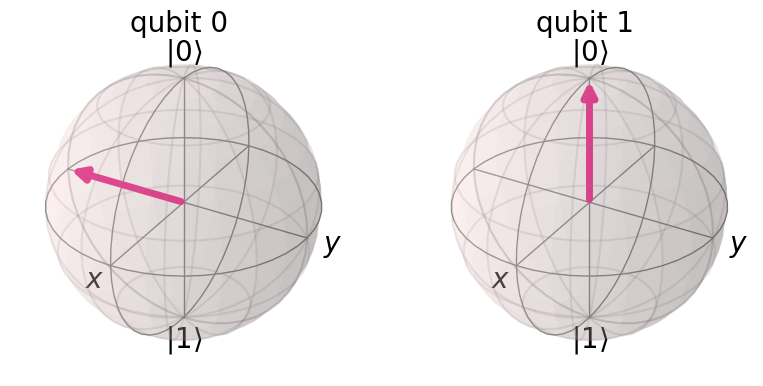
\includegraphics[width=0.3\textwidth]{1g.png}
\caption{\label{fig:frog}1(g) bloch sphere.}
\end{figure}

\subsection{(h)}
\begin{enumerate}
    \item Try to prepare a qubit state with $Prob(1) = \frac{2}{3}$
    \item Then apply Hadamard gate to transform its basis to x basis
    \item Detailed code as below:
    \begin{lstlisting}[language=Python]
    q = QuantumRegister(1)
    c = ClassicalRegister(1)
    ckt = QuantumCircuit(q,c)
    pi = math.pi
    ckt.rx(2*pi/3,q[0])
    ckt.h(q[0])
    def x_mesaurement(qc,qubit,cbit):
       qc.h(qubit)
       qc.measure(qubit,cbit)
       return qc
    sim = Aer.get_backend('aer_simulator')
    x_mesaurement(ckt,0,0)
    ans = assemble(ckt)
    counts = sim.run(ans).result().get_counts()  
    plot_histogram(counts)
    \end{lstlisting}
    which I get $Prob(+) = 0.270,Prob(-) = 0.730$
    
\end{enumerate}

\section{Manipulating Multi-Qubit Gates}
\subsection{(a)} 
I get $Prob(00) \approx Prob(01) \approx Prob(10) \approx Prob(11) \approx 0.25$

\subsection{(b)}
After the Hadamard, cnot gates and the measurement,I get $Prob(00) \approx Prob(11) \approx 0.5$. which proves that the qubit is in maximally entangled state

\subsection{(c)}
After trying the circuit, the outcome is $Prob(00) \approx Prob(01) \approx Prob(10) \approx Prob(11) \approx 0.25$ ,which can slightly imply that we gain $Prob(++) \approx Prob(--)  \approx 0.5$

\subsection{(d)}
The other three Bell states are prepared as below
\begin{enumerate}
    \item $\phi-$ 
    \begin{lstlisting}[language=Python]
    qphi_minus = QuantumCircuit(2)
    qphi_minus.x(0)
    qphi_minus.h(0)
    qphi_minus.cnot(0,1)
    \end{lstlisting}
    which ends in the state vector as 
    $Statevector =\begin{bmatrix}
    \frac{1}{\sqrt{2}} & 0 & 0 & - \frac{1}{\sqrt{2}}
    \end{bmatrix} $
    \item $\psi+$  
    \begin{lstlisting}[language=Python]
    qpsi_plus = QuantumCircuit(2)
    qpsi_plus.x(1)
    qpsi_plus.h(0)
    qpsi_plus.cnot(0,1)
    \end{lstlisting}
    which ends in the state vector as 
    $Statevector =\begin{bmatrix}
    0 & \frac{1}{\sqrt{2}} & \frac{1}{\sqrt{2}} & 0
    \end{bmatrix} $
    \item $\psi-$ 
    \begin{lstlisting}[language=Python]
    qpsi_minus = QuantumCircuit(2)
    qpsi_minus.x(0)
    qpsi_minus.x(1) 
    qpsi_minus.h(0)
    qpsi_minus.cnot(0,1)
    \end{lstlisting}
    which ends in the state vector as 
    $Statevector =\begin{bmatrix}
    0 & -\frac{1}{\sqrt{2}} & \frac{1}{\sqrt{2}} & 0
    \end{bmatrix} $
    
\end{enumerate}
\subsection{(e)}
I prepared

\section{Global phase does not matter}
\subsection{(a)}
After the two circuits, the vector representation in computational basis of each outcomes are as below respectively

$\phi1 = \begin{bmatrix}
    \frac{1}{\sqrt{2}} & \frac{1}{\sqrt{2}} 
    \end{bmatrix}$
, $\phi2 = \begin{bmatrix}
    -\frac{i}{\sqrt{2}} & -\frac{i}{\sqrt{2}} 
    \end{bmatrix}$
    
But the measurement outcomes are both $Prob('0') \approx Prob('1') \approx 0.5$. This refers that the two circuits can't be distinguished by measurement outcomes.

\subsection{(b)}
I used U gate to create two qubits that only differ from global phases, detailed code as below
\begin{lstlisting}[language=Python]
pi = math.pi
psi1 = QuantumCircuit(1)
psi1.u(pi/3,pi/3,0,0) # psi2 is created similarly as psi2.u(pi/3,pi/2,0)
\end{lstlisting}
After the two circuits, the vector representation in computational basis of each outcomes are as below respectively

$\phi1 = \begin{bmatrix}
    \sqrt{\frac{3}{4}} & \frac{1}{4}+0.43301i 
    \end{bmatrix}$
, $\phi2 = \begin{bmatrix}
    \sqrt{\frac{3}{4}} & \frac{i}{2} 
    \end{bmatrix}$
But the measurement outcomes are both $Prob('0') \approx 0.3, Prob('1') \approx 0.7$. This refers that the two circuits can't be distinguished by measurement outcomes.
\subsection{(c)}
After the two circuits, the vector representation in computational basis of each outcomes are as below respectively

$\phi1 = \begin{bmatrix}
    \frac{1}{\sqrt{2}} & -\frac{1}{\sqrt{2}} 
    \end{bmatrix}$
, $\phi2 = \begin{bmatrix}
    \frac{1}{\sqrt{2}} & \frac{1}{\sqrt{2}} 
    \end{bmatrix}$
But the measurement outcomes are both $Prob('0') \approx Prob('1') \approx 0.5$. This refers that the two circuits can't be distinguished by measurement outcomes.
But it still can't be considered as equivalent,because that it's only a coincidence in this case that the measurement outcomes are quite similar. 
\section{The Swap test}
\begin{enumerate}
    \item If the two states are the same, the outcome I gain is $Prob('1') = 1$
    \item If the two states are orthogonal, the outcome I gain is $Prob('0') \approx
    Prob('1') \approx 0.5$
    \item If the two states are different, the outcome I gain is depend on their similarities, in the example I use $Prob('0') \approx 0.12 ,
    Prob('1') \approx 0.88$
    \item The three tests have similar codes, which I only present one as below
    \begin{lstlisting}[language=Python]
    sqrt = math.sqrt
    q4 = QuantumRegister(3)
    c4 = ClassicalRegister(1)
    ckt4 = QuantumCircuit(q4,c4)
    #ckt4.x(q4[1]) (If we want orthogonal cases)
    #ckt4.u(pi/30,pi/4,0,q4[0])(If we want different cases)
    #ckt4.u(pi/3,pi/4,pi/3,q4[1])(If we want different cases)
    ckt4.h(q4[2])
    ckt4.cswap(q4[2],q4[1],q4[0])
    ckt4.h(q4[2])
    ckt4.x(q4[2])
    ckt4.measure(q4[2],c4)
    simulator = Aer.get_backend('aer_simulator')
    job = execute(ckt4, simulator, shots = 1024)
    result = job.result()
    counts = result.get_counts()
    \end{lstlisting}
    \item By Swap Test, if the two qubits are indeed the same up to global phase,the states can't be tell.
    
\end{enumerate}
\section{ Quantum Random Number Generator}
\subsection{(a)}
Using the randomness of qubit states, I prepare a qubit state as $ \mid + \succ$ by applying hadamard state, then I used n measurements to gain n outcomes (the outcomes have $Prob(0) \approx Prob(1) \approx 0.5$,which means it randomly decide the current bit) and append it into a bitstring which I can convert it back to an integer. Detailed code are shown below
\begin{lstlisting}[language=Python]
q5 = QuantumRegister(1)
c5 = ClassicalRegister(1)
ckt5 = QuantumCircuit(q5,c5)
ckt5.h(q5[0])
ckt5.measure(q5,c5)
simulator = Aer.get_backend('qasm_simulator')
def QRNG(n):
    ans = ''
    for i in range(n):
        job = execute(ckt5, simulator, shots = 1)
        result = job.result()
        counts = result.get_counts()
        for key,value in counts.items():
            temp = key
            ans+=str(key)
    return ans
bit_length = int(input())
ans = QRNG(bit_length)
print(int(ans,2))
\end{lstlisting}
The sequence output of the QRNG(4) I designed is 5,4,13,0,6,11,3,12,9,1.Yes,they are random by the probability that the outcomes of every bit is $Prob(0) \approx Prob(1) \approx 0.5$,which means it every number has prob. = $\frac{1}{16}$
\subsection{(b)}
The answer is the same as above,it successfully creates random sequences, and the sequence that my function created is 1,5,13,7,14,3,7,9,11,2,4.
\end{CJK*}
\end{document}
